\documentclass[a4paper]{article} 
\input{style/head.tex}

%-------------------------------
%	TITLE VARIABLES (identify your work!)
%-------------------------------

\newcommand{\yourname}{PICARD Emilio} % replace YOURNAME with your name
\newcommand{\youremail}{emilio.picard@free.fr} % replace YOUREMAIL with your email
\newcommand{\assignmentnumber}{4} % replace X with the lab session number

\begin{document}

%-------------------------------
%	TITLE SECTION (do not modify unless you really need to)
%-------------------------------
\input{style/header.tex}

%-------------------------------
%	ASSIGNMENT CONTENT (add your responses)
%-------------------------------

\section*{Question 1}
Let define $G_1$ and $G_2$ as the two connected components
described in the question. Define $N_1$ and $N_2$ as $N_1 = 100$ and $N_2 = 50$.
\subsubsection*{Number of edges in $G$}
In $G_1$, the number of edges is $\binom{N_1}{2} = \frac{N_1(N-1)}{2} = 4950$.
\\
In $G_2$, the number of edges is $N_2 \times N_2$ as $G_2$ is a bipartie graph where
each partition set has $N_2$ vertices. Thus, the number of edges in $G_2$ is $N_2 \times N_2 = 2500$.
Finally, the total number of edges in $G$ is $4950 + 2500 = 7450$.

\subsubsection*{Number of triangles in $G$}
In $G_1$, the number of triangles is $\binom{N_1}{3} = \frac{N_1(N_1-1)(N_1-2)}{3\times2} = 161700$.
\\
In $G_2$, the number of triangles is $0$ because it is a complete bipartite graph.\\
Finally, the total number of triangles in $G$ is $161700$.

\section*{Question 2}
\textbf{For subfigure (a):}
\\
In the proposed graph, we can observe two different communities (clusters),
the green one with nodes $\{1, 2, 3, 4, 5\}$ and the blue one with nodes $\{6, 7, 8, 9\}$.
We thus have $n_c=2$.
To compute the modularity metric, we need to compute the number of edges inside each community ($l_1$ and $l_2$),
the total number of edges of the whole graph ($m$) and the sum of the degrees of each nodes inside a community($d_1$ and $d_2$).
\\
\\
We observe that:
\begin{itemize}
    \item $m = 13$
    \item $l_1 = 6$ and $l_2 = 6$
    \item $d_1 = 13$ and $d_2 = 13$
\end{itemize}
Thus, the modularity metric is:
\begin{align*}
    Q &= \left(\frac{l_1}{m} - \left(\frac{d_1}{2m}\right)^2\right) + \left(\frac{l_1}{m} - \left(\frac{d_1}{2m}\right)^2\right) \\
    &= \left(\frac{6}{13} - \left(\frac{13}{26}\right)^2\right) + \left(\frac{6}{13} - \left(\frac{13}{26}\right)^2\right) \\
    &= \frac{6}{13} - \frac{1}{4} + \frac{6}{13} - \frac{1}{4} \\
    &= \frac{12}{13} - \frac{1}{2} \\
    &= \frac{24}{26} - \frac{13}{26} \\
    &= \frac{11}{26} \in [-1, 1].
\end{align*}
\\
\\
\textbf{For subfigure (b):}
\\
Using the same method as for subfigure (a), we have:
\begin{itemize}
    \item $m = 13$
    \item $l_1 = 2$ and $l_2 = 4$
    \item $d_1 = 11$ and $d_2 = 15$
\end{itemize}
Thus, the modularity metric is:
\begin{align*}
    Q &= \left(\frac{2}{13} - \left(\frac{11}{26}\right)^2\right) + \left(\frac{4}{13} - \left(\frac{15}{26}\right)^2\right) \\
    &= \frac{2}{13} - \frac{121}{676} + \frac{4}{13} - \frac{225}{676} \\
    &= \frac{6}{13} - \frac{346}{676} \\
    &= \frac{6}{13} - \frac{173}{338} \\
    &= \frac{156}{338} - \frac{173}{338} \\
    &= -\frac{17}{338} \in [-1, 1].
\end{align*}

\section*{Question 3}
For $n=4$, let $P_4$ be:
\begin{figure}[ht]
    \centering
    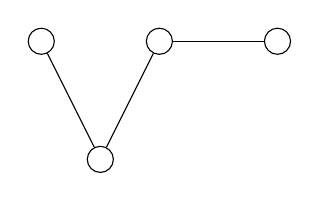
\begin{tikzpicture}
        \node[circle, draw, fill=white] (A) at (0, 1.5) {};
        \node[circle, draw, fill=white] (B) at (0.75, 0) {};
        \node[circle, draw, fill=white] (C) at (1.5, 1.5) {};
        \node[circle, draw, fill=white] (D) at (3, 1.5) {};
        \draw (A) -- (B);
        \draw (B) -- (C);
        \draw (C) -- (D);
    \end{tikzpicture}
    \caption{$P_4$}
\end{figure}

and $C_4$ be:
\begin{figure}[ht]
    \centering
    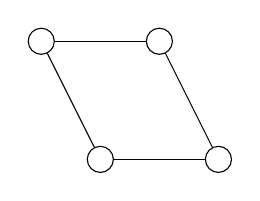
\begin{tikzpicture}
        \node[circle, draw, fill=white] (A) at (0, 1.5) {};
        \node[circle, draw, fill=white] (B) at (0.75, 0) {};
        \node[circle, draw, fill=white] (C) at (2.25, 0) {};
        \node[circle, draw, fill=white] (D) at (1.5, 1.5) {};
        \draw (A) -- (B);
        \draw (B) -- (C);
        \draw (C) -- (D);
        \draw (D) -- (A);
    \end{tikzpicture}
    \caption{$C_4$}
\end{figure}

for $C_4$:
\begin{itemize}
    \item 4 paths of length 1
    \item 2 paths of length 2
    \item 0 paths of length 3
\end{itemize}

for $P_4$:
\begin{itemize}
    \item 3 paths of length 1
    \item 2 paths of length 2
    \item 1 paths of length 3
\end{itemize}

To compute the shortest path kernel between 2 graphs, we need to compute the inner product between the two feature vectors..
Doing though for all lengths, we get the following kernels:
$$
    k(P_4, C_4) = 3 \times 4 + 2 \times 2 + 1 \times 0 = 16.
$$
$$
    k(C_4, C_4) = 4 \times 4 + 2 \times 2 = 20.
$$
$$
    k(P_4, P_4) = 3 \times 3 + 2 \times 2 + 1 \times 1 = 14.
$$
\section*{Question 4}
Let $G$, $ G^{'}$ be two undirected graphs. Let $\mathcal{G} = \{graphlet(1), \dots, graphlet(N_3)\}$,
with $N_3 = 4$. With the notations of the question and the article \cite{pmlr-v5-shervashidze09a},
let $f_G$ (respectively $f_{G^{'}}$) be a vector of length $N_3$, whose $i^{th}$
component is the number of occurence of $graphlet(i)$ in $G$ (respectively in $G^{'}$).
The graphlet kernel is defined as $$k(G, G^{'}) = f_G^\top f_{G^{'}}.$$

If $k(G, G^{'}) = 0$, it means that $f_G^\top f_{G^{'}} = 0$, so $f_G$ and $f_{G^{'}}$
are orthogonal. As $\forall i \in \{1, \dots, N_3\}, \forall G,  f_G^i \geq 0$ (denoting $f_G^i$ as the $i^{th}$
component of vector $f_G$), the only possibility for $k$ to be equal to $0$ is
that $\forall i, f_G^i f_{G^{'}}^i = 0$. This implies that there is no similar graphlets
between the compared graphs (they don't have any common subgraphs structure).
\\
However, it is possible that a 3-size graphlet kernel can lead to a zero value,
rather that a 4-size graphlet kernel can capture similarities (between the same graphs).
This can happens because of a graph complexity.
\\
\\
\textbf{Example of two graphs $G$ and $G^{'}$ which $k(G, G^{'})=0$:}
\\
For a 3-size kernel: the 4 different graphlets are represented in figure \ref{fig:graphlet-size-3}.

\begin{figure}[ht]
    \centering
    
    \begin{subfigure}{0.22\textwidth}
        \centering
        
\begin{tikzpicture}
            \node[circle, draw, fill=white] (A) at (0, 0) {};
            \node[circle, draw, fill=white] (B) at (1.5, 0) {};
            \node[circle, draw, fill=white] (C) at (3, 0) {};
        \end{tikzpicture}
        \caption{Isolated nodes}
    \end{subfigure}
    \hspace{0.3cm}
    \begin{subfigure}{0.22\textwidth}
        \centering
        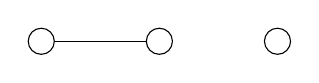
\begin{tikzpicture}
            \node[circle, draw, fill=white] (A) at (0, 0) {};
            \node[circle, draw, fill=white] (B) at (1.5, 0) {};
            \node[circle, draw, fill=white] (C) at (3, 0) {};
            \draw (A) -- (B);
        \end{tikzpicture}
        \caption{One edge}
    \end{subfigure}

    \vspace{0.5cm}
    \begin{subfigure}{0.22\textwidth}
        \centering
        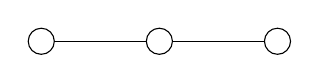
\begin{tikzpicture}
            \node[circle, draw, fill=white] (A) at (0, 0) {};
            \node[circle, draw, fill=white] (B) at (1.5, 0) {};
            \node[circle, draw, fill=white] (C) at (3, 0) {};
            \draw (A) -- (B);
            \draw (B) -- (C);
        \end{tikzpicture}
        \caption{Path of 3 nodes}
    \end{subfigure}
    \hspace{0.5cm}
    \begin{subfigure}{0.22\textwidth}
        \centering
        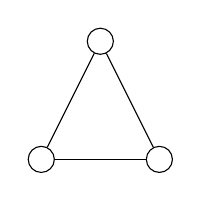
\begin{tikzpicture}
            \node[circle, draw, fill=white] (A) at (0, 0) {};
            \node[circle, draw, fill=white] (B) at (1.5, 0) {};
            \node[circle, draw, fill=white] (C) at (0.75, 1.5) {};
            \draw (A) -- (B);
            \draw (B) -- (C);
            \draw (C) -- (A);
        \end{tikzpicture}
        \caption{Triangle}
    \end{subfigure}
    
    \caption{The four different graphlets of size 3}
    \label{fig:graphlet-size-3}
\end{figure}


Let's choose two undirected graphs $G$ and $G^{'}$:
\begin{figure}[ht]
    \centering
    \begin{subfigure}{0.22\textwidth}
        \centering
        
\begin{tikzpicture}
            \node[circle, draw, fill=white] (A) at (0, 0) {};
            \node[circle, draw, fill=white] (B) at (1.5, 0) {};
            \node[circle, draw, fill=white] (C) at (3, 0) {};
        \end{tikzpicture}
        \caption{Graph $G$}
    \end{subfigure}
    \hspace{0.5cm}
    \begin{subfigure}{0.22\textwidth}
        \centering
        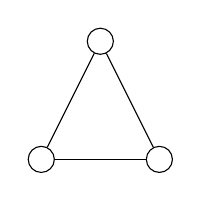
\begin{tikzpicture}
            \node[circle, draw, fill=white] (A) at (0, 0) {};
            \node[circle, draw, fill=white] (B) at (1.5, 0) {};
            \node[circle, draw, fill=white] (C) at (0.75, 1.5) {};
            \draw (A) -- (B);
            \draw (B) -- (C);
            \draw (C) -- (A);
        \end{tikzpicture}
        \caption{Graph $G^{'}$}
    \end{subfigure}
    \caption{}
    \label{fig:graphs}
\end{figure}

Let's compute the graphlet kernel between $G$ and $G^{'}$:
\begin{align*}
    k(G, G^{'}) &= f_G^\top f_{G^{'}} \\
    &= \begin{pmatrix} 1 & 0 & 0 & 0 \end{pmatrix} \begin{pmatrix} 0 \\ 0 \\ 0 \\ 1 \end{pmatrix} \\
    &= 0.
\end{align*}


%------------------------------------------------

\bibliographystyle{plain}
\bibliography{references} % citation records are in the references.bib document

\end{document}
